Consider the left image in Figure \ref{fig:introPhoto}. Even though the person on the right is comparable in size to the person on the left, he is remembered far less by human subjects, indicated by their respective memorability scores of $0.18$ and $0.64$. Moreover, people tend to remember the person on the left and the fish in the center, even after $3$ minutes and  more than 70 additional visual stimuli have passed. Interestingly, despite vibrant colors and considerable size, the boat is far less memorable with a memorability score of $0.18$.

\begin{figure}[t]
\centering
\subfigure{\centering 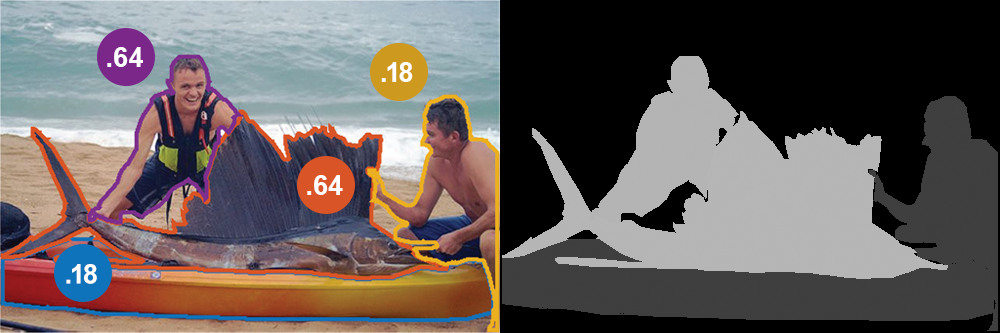
\includegraphics[width=0.475\textwidth]{figures/introduction/front_page.png}}
\vspace{-12pt}\caption{\footnotesize\textbf{Not all objects are equally remembered.} Image showing objects and their respective memorability scores (left) obtained from our experiment. We note that certain objects (the fish and left person) are more memorable than other objects. Right figure shows the ground truth map generated from the object segments and memorability scores.}\label{fig:introPhoto}\vspace{-15pt}
\end{figure}


One of the primary goals of computer vision is to aid human-relevant tasks, such as object recognition, object detection, and scene understanding. Much of the algorithms in service of this goal have to make inferences about all objects in a scene. In comparison, humans are incredibly selective in the information they consider from the possible visual candidates they experience, and as a result, many human tasks are dependent on this filtering mechanism to be performed effectively. For this reason, it is important for vision systems to have information on hand concerning what objects humans deem important in the world, or in our specific case, which of them are worth remembering. Such information holds exciting promise. For example, it can enrich instructional designs for education, so as to maximize a student's retention while minimizing distractions, as well as, enable intelligent ad placement software that embeds adverts in images and videos in such a way that humans are likely not to forget.

Going back to Figure \ref{fig:introPhoto}, why are the fish and left person more memorable and how do these objects influence the overall memorability of the photo? The field has made great strides in understanding comparable visual  properties of the world such as saliency \cite{it} and importance \cite{berg12} value, but we still do not have a clear understanding of what objects are ``worth” remembering in the world. Although recent studies related to image memorability \cite{isola11,isola11nips,khosla13,isola14,zoya15} have explored this at the image-level, no work has explored what exactly in an image is remembered. Using object annotations and predictive models, such knowledge can be potentially inferred from the memorability score of an image alone \cite{khosla12}, but these methods will ultimately require ground truth object memorability data to be properly evaluated and analyzed. To enable the development of such approaches, we collect ground truth object-level memorability scores and conduct an extensive empirical investigation of  memorability at the object-level, a simple yet powerful strategy that provides detailed answers to many interesting questions at hand. While image memorability studies have provided invaluable knowledge, the study of object memorability in images not only sheds light on what elements of an image are remembered, but it also should eventually put forth, by its very nature, a bottom-up account of memorability. More importantly, such an analysis will enable unique applications in the fields of computer vision and computational photography not possible from the study of image memorability alone.

In this paper, we systematically explore the memorability of objects within individual images and shed light on the various factors that drive object memorability. In exploring the connection between object memorability, saliency, object categories, and image memorability, our paper makes several important contributions.

\vspace{3pt}\noindent\textbf{Contributions.} \textbf{(1)} This paper presents the first work that studies the problem of object memorability and provides a deeper understanding of what makes objects in an image memorable or forgettable. While previous work has tried to infer such knowledge  computationally \cite{khosla12}, our work is the first to directly quantify and study what objects in an image humans actually remember.  \textbf{(2)} We uncover the relationship between visual saliency and object memorability and demonstrate those instances where visual saliency directly predicts object memorability and when/why it fails to do so. While there have been a few very recent studies that explore the connection between image memorability and visual saliency \cite{zoya15,lemeur13,kim13}, our work is the first to explore the connection between object-level memorability and visual saliency. %To the best of our knowledge, our work is the first to show the differences and overlap between saliency and memorability and how the two phenomena differ from each other.  
\textbf{(3)} We make significant headway in disambiguating the link between image and object memorability. We show that in many cases, the memorability of an image is primarily driven by the memorability of its most memorable object. %Studying these questions helps us not only understand visual saliency, image and object memorability in more detail, but it can also have important contributions to computer vision. For example, understanding which regions and objects in an image are memorable would enable us to modify the memorability of images which can have applications in advertising, user interface design, etc. 
Furthermore, we show that our compiled dataset can serve as a benchmark for evaluating automated object memorability algorithms and enable/encourage future work in this exciting line of research.%object and region memorability prediction schemes.
